\documentclass[letterpaper]{article}
\usepackage{natbib,alifexi}
\usepackage[utf8x]{inputenc}

\usepackage{xcolor}

\title{Plan-Based Reward Shaping for Multi-Agent Reinforcement Learning}
\author{Jérôme Bastogne$^{1}$, Maxime Desclefs$^{1}$ \and Simon Picard$^{1}$ \\
\mbox{}\\
$^1$Université Libre de Bruxelles, Boulevard du Triomphe - CP 212, 1050 Brussels, Belgium \\
jbastogn@ulb.ac.be, mdesclef@ulb.ac.be, spicard@ulb.ac.be}


\begin{document}
\maketitle

\begin{abstract}
Reward shaping is known to significantly improve an agent’s performance in multi-agent reinforcement
learning (MARL). This paper shows the benefits of using plan-based reward shaping in which a STRIPS planning knowledge is used. The results of agents using plan-based reward shaping will then be compared to a simple Reinforcement Learning (RL) agent with no domain knowledge and they will show how they outperform previous results.
\end{abstract}

\section{Introduction}

Reinforcement learning agents don't get future feedback about how good was their decision taken in a precise state. This leads to a temporal problem as the agents will not know immediately which part of their decisions where the good ones \citep{rs}. RL, while being simple, presents some issues. The time taken by the agents to learn the right policy grows exponentially while adding new variables to the environment. When the state space is too vast, memory becomes an issue as well as the matrix for each state-action pair becomes too big and too many states need to be updated too frequently slowing down drastically the process. 

A way of improving the converging speed is to provide prior knowledge to the agents through a method called reward shaping. Reward shaping is the addition of domain knowledge to reinforcement learning in a way that will minimize non-optimal behaviours and will fastly converge to the optimal one. In this article we will see how to effectively incorporate reward shaping in MARL using individual and joint plan based plans and we will combine them with a flag based heuristic\citep{paper4}.

We will show that providing prior knowledge, while not always being possible due to heuristic problems, significantly increases agent's performances and speed of convergence.


\section{Materials and Methods}
\subsection{Reinforcement Learning}
Reinforcement learning is a method of rewarding an agent for taking a good decision in a particular state. The better state the decision leads to, the better that decision will be rewarded. Therefore RL can be considered as a Markov Decision Process. Each agent remembers what rewards he got for each action in each state. 

The possible actions here are going up, down, left and right. A state here, is a position (x, y) in the world space combined the current step in the plan. To each of these Q(s,a )state-action pairs is associated a Q-value translating the goodness of choosing that action while being in that state. The reinforcement algorithm is iterative and dynamic, therefore agents have to run multiple episodes where they have to reach the goal and where they are rewarded depending on the number of flags they got together. At each step, we need to update Q(s,a)  for future learning. A way of achieving this is by applying a temporal-difference update to Q(s,a) so that Q(s,a) will increase only if it leads to a better state than the actual one. This ensures that agents are willing of doing better while reaching the goal. There is an algorithm called SARSA that does this by updating Q-values as follows : \\

$Q(s, a) \leftarrow  Q(s, a) +  \alpha [r + \gamma Q(s', a') - Q(s,a)]$\\\\
where $\alpha$ is the rate of learning and $\gamma$ is the discount factor. r is the reward returned by the environment. In our case, reward will only be given when agents reach the goal. 

At start, agents know nothing about their environment therefore they will randomly travel through the world space. After few iterations some of their actions will have positive rewarded scores but might not be the most optimals. Therefore, a good balance between exploration and exploitation of the best rewarded actions must be found. The most common method is by using the $\epsilon$-greedy algorithm. It ensures that at each step, the best value action will be chosen with a probability 1- $\epsilon$ and otherways the agent will explore a new action.


A well-known method to fasten this process is eligibility traces. When a reward is received, the lasts state-actions pairs that the agent has been walking through are also updated according to their temporal difference with the last state-action pair. Each Q-value is updated as follows : \\

$Q(s, a) \leftarrow  Q(s, a) +  \alpha *  \sigma (\gamma * \lambda)^t$\\\\
where $\lambda$ has to be lower or equal to 1 \citep{etrace}. We choosed  $\lambda = 0.4$ for our experiment.

\subsection{Plan-Based Reward Shaping}

The addition of reward shaping to reinforcement learning changes the SARSA algorithm formula as follows: \\

$Q(s, a) \leftarrow  Q(s, a) +  \alpha [r + F(s, s') + \gamma Q(s', a') - Q(s,a)]$\\\\
where $ F(s, s')$  is a difference of potentials defined as follows : \\

$F(s, s') =\gamma \phi (s') - \phi (s)$\\\\
where $\phi$ is some function over states. The difference of potentials is usefull for avoiding cycles  \citep{rs2}.

For plan-based reward shaping, agents are given STRIPS plans that transposes into a list of states. The agent's potential $\phi$ can be chosen as :\\

$\phi (s) = \omega * CurrentStepInPlan$\\\\
where $\omega$ is a scaling factor and $CurrentStepInPlan$ is the corresponding plan's step of the agent's state.

\section{Study Case}

\begin{figure}[h!]
  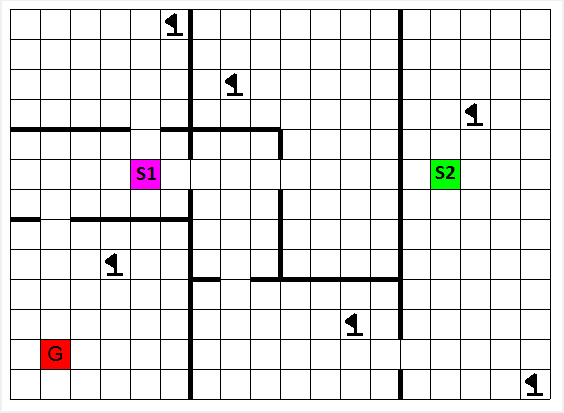
\includegraphics[width=\linewidth]{img/studycase.png}
  \caption{Multi-Agent, Flag-Collecting Problem Domain.}
  \label{fig:studycase1}
\end{figure}





\section{Results and Discussion}
\section{Conclusion}




\footnotesize
\bibliographystyle{apalike}
\bibliography{example}


\end{document}
